\section{Introduction}
\label{sec:introduction}

Large language models have made it possible to construct agents that read
natural-language situations, plan, and write socially legible actions.  This
capability has renewed interest in \emph{generative agents} and in
\emph{LLM-based social simulation}
\citep{park2023generative,park2024grounded,argyle2023outofone}, but a
persuasive conversation is not yet an artificial society.  A research-grade
artificial society must let its inhabitants persist across simulated time, act
from shared locations and relations, encounter consequences of earlier
decisions, and leave evidence from which a researcher can reconstruct what
happened.  The mechanisms that surround the language model---time, space,
exposure, institutions, resource constraints, audit, and intervention---must
be explicit enough to inspect and vary.  This is a systems problem, not a
prompt-crafting problem.

GAWorld is research infrastructure for building such societies.  The first
arXiv system paper froze the audited K1--K5 microkernel state of the codebase
at a single repository commit and reported nine built-in plugins, an artifact
ledger, and a single-tenant, single-process deployment model
\citep{gawoerldv1}.  Since that snapshot, the system has been extended in five
directions that, taken together, change what the platform is for:

\begin{enumerate}[leftmargin=*,label=\textbf{\arabic*.}]
  \item \textbf{Plugin breadth and surface closure.}  The built-in plugin set
  has grown from nine to fourteen; new plugins add personality-grounded
  behavior, dynamic interruption rules, indoor room resolution, an
  information-diet that mixes agent-derived queries with external sources, and
  organizational governance.  Each plugin either participates through the
  event bus or is admitted as a built-in whose semantics are documented.
  \item \textbf{Multi-tenant worlds.}  A persistent account store with
  invite-code registration, role-based membership, per-world configuration
  overlays, copy-on-write city bundles, per-tenant quotas, and audit trails
  lets a single deployment host many independent societies with different
  visibility.  When the account store is absent the system reverts, byte for
  byte, to its single-tenant behavior.
  \item \textbf{Distributed execution and playable cities.}  A world may be
  partitioned across a hub and many nodes: the hub owns accounts, the world
  metadata, and the players; each node runs its assigned inhabitants with its
  own model key.  Players can enter an \emph{open} world through a browser
  lease, claim a resident, and act in the next tick; a strict intervention
  outbox routes their actions to the right node.  This is a deployment
  primitive, not a claim of high-throughput distributed simulation.
  \item \textbf{Research and counterfactual workflow.}  Beyond the
  matched-event workflow, the stack adds a parallel-worlds engine that runs up
  to eight matched worlds across multiple seeds, a Research Workbench that
  compiles a paper or research idea into a pre-registered protocol, an
  Agent Arena for benchmarking residents, a policy simulation and optimization
  loop, and a serious-game workshop.  Each result is bound to a hash, a
  record of completion, and an evidence class.
  \item \textbf{Persona distillation and population work.}  A name or a URL
  can be distilled into a sourced portrait that becomes a resident plus a
  reusable mental-model skill; offline citizens, families, organizations, and
  bulk imports now coexist with online ones.  The City API and Agent Studio
  expose population construction as a first-class activity.
\end{enumerate}

The platform has also internalized the lessons of its first audit.  Where
v1 distinguished implementation visibility from empirical validity, v2 adds
explicit evidence classes (\textsf{REAL}, \textsf{DIAGNOSTIC},
\textsf{SYNTHETIC}, \textsf{INCOMPLETE}, \textsf{DESIGNED}, \textsf{FIXTURE}) and
insists that every reported number carry an evidence class and a hash.  Where
v1 described a single notebook, v2 separates a self-contained harness
(\textsf{GAWorld-Bench Track~A}, software-path diagnostics) from a gameplay
probe library (\textsf{Track~B}, judgement-based evaluation).  Where v1
described a single, frozen migration, v2 describes an open engineering frontier
together with the current migration status of each subsystem.

This paper makes five contributions:

\begin{enumerate}[leftmargin=*,label=\textbf{C\arabic*.}]
  \item \textbf{An integrated, plugin-bounded research stack.}  We describe
  the v2 architecture, the boundary between the kernel and the
  domain-owned plugins, and the event-bus semantics that lets mechanisms
  observe, contribute, and filter at defined lifecycles.  The architecture
  covers 14 built-in plugins, an agent step pipeline of 12 stages, a
  per-tenant world path resolver, a distributed hub-and-node protocol, and a
  parallel-worlds engine.

  \item \textbf{Multi-tenant, multi-machine, playable societies.}  We show how
  a single deployment hosts a classroom, a research group, and a
  cross-machine run from the same codebase, with per-world isolation,
  per-tenant quotas, role-based visibility, and a hub-node message relay that
  routes player interventions to the correct node in at most one tick.

  \item \textbf{An inspectable, evidence-classed experimental workflow.}  We
  integrate matched-event, parallel-worlds, paper-to-protocol, policy
  optimization, and gameplay-based evaluation under a single evidence ledger
  with hash-bound artifacts.  Each research question has a permitted claim
  class, and each numerical result carries the evidence class and the
  producing code path.

  \item \textbf{Behavior realism and societal substrate.}  We describe the
  persistent state, the Big-Five personality plugin, the dynamic-interruption
  module, the spatial tree that brings indoor rooms into the simulation, the
  endogenous inflation and credit-bound consumption model, the
  organizational-governance engine, and the offline-resident taxonomy.

  \item \textbf{Validation, reproducibility, and ethical boundaries.}  We
  report the same five-claim validation framework as v1, expanded to
  accommodate the new evidence classes and the new research surfaces, and
  we map the engineering and research roadmaps onto the boundary between
  software progress and substantive social-scientific claim.
\end{enumerate}

\begin{figure}[t]
  \centering
  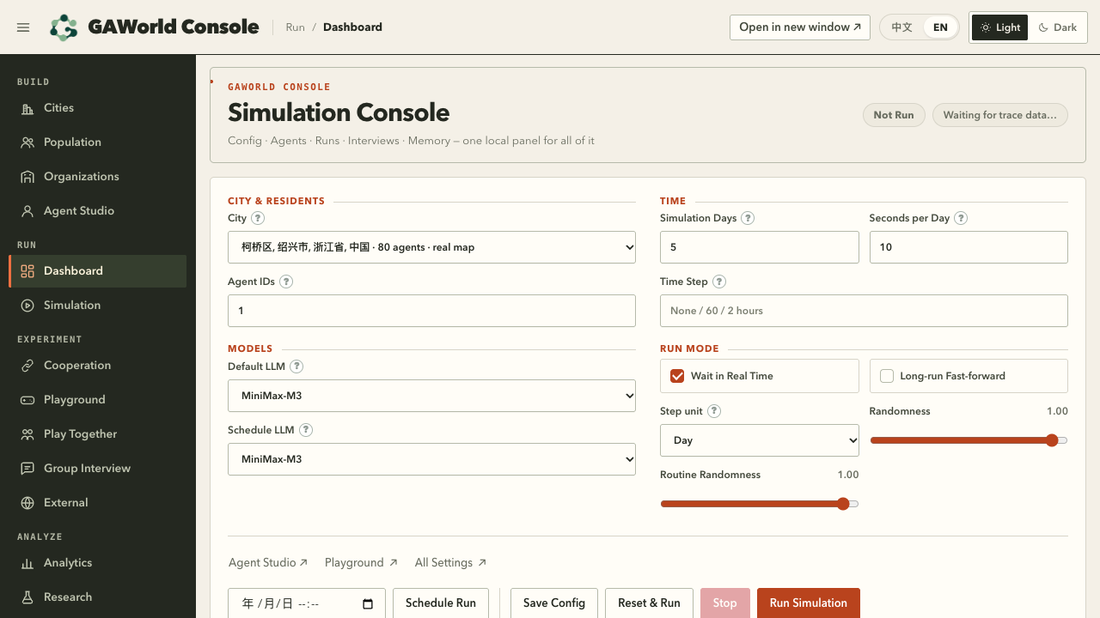
\includegraphics[width=\linewidth]{en_01_console.png}
  \caption{The GAWorld Console.  The left navigation exposes every
  v2 surface: \emph{Cities} and \emph{Population} build the city bundle;
  \emph{Organizations} edits rules and members; \emph{Agent Studio} shapes
  individual residents; the \emph{Dashboard} (shown) configures and starts a
  run; the \emph{Playground}, \emph{Play Together}, and \emph{Group Interview}
  tabs run game-based probes, an open-world player lease, and one-shot
  elicitation; \emph{External} drives the relay and external-environment
  services; and \emph{Analytics} / \emph{Research} surface the result
  inspection and the counterfactual / paper-to-protocol workflows.  The
  screenshot was captured against the bundled Keqiao (Shaoxing) city bundle
  in single-tenant, single-process mode; the dashboard UI was switched to
  English via \texttt{window.setLocale('en')}, while the resident content
  reflects the language of the bundled data.}
  \label{fig:console}
\end{figure}

GAWorld v2 is presented as a configurable scientific instrument, not as a
representative synthetic population, a digital twin, or a forecasting
system.  Its artifacts do not establish that generated agents reproduce
particular people, that aggregate trajectories match a real city, or that a
simulated intervention estimates a real policy effect.  We instead treat the
system as an instrument whose outputs are evaluated at five claim levels
(individual consistency, macro correspondence, emergent dynamics,
counterfactual response, reproducibility) and whose evidence ledger is a
prerequisite for substantive interpretation.

The remainder of the paper proceeds as follows.  \Cref{sec:design-goals}
states the design goals; \Cref{sec:related-work} positions v2 against
generative agents, language agents, social evaluation, agent-based modeling,
and platform research.  \Cref{sec:agent-lifecycle,sec:microkernel,sec:memory-cognition-realism}
describe the agent, the kernel, and the cognitive substrate.
\Cref{sec:substrate,sec:multi-user-worlds,sec:distributed-playable} describe
the societal substrate, multi-tenancy, and the distributed playable runtime.
\Cref{sec:research-workflow,sec:playground-arena} describe the research and
gameplay surfaces.  \Cref{sec:capability-cases,sec:validation-boundaries}
audit the existing capability cases against the five claim levels.
\Cref{sec:limitations-ethics-roadmap} states the limits and the roadmap.
\Cref{sec:conclusion} concludes.
